\subsection{Mathematik}

\subsubsection{Berechnung der Solarzellenkennlinie}

Gemäss \colorbox{red}{Quelle: Photovoltaik Engineering} lässt sich die Kennlinie der Solarzelle aus folgenden Parametern berechnen:
\begin{align*}
	I_{SC} &= 3.09A \\
	U_{OC} &= 22.0V \\
	I_{Pmax} &= 2.90A \\
	U_{Pmax} &= 18.0V
\label{eq:eingangsparameter_kennlinie}
\end{align*}

Mit diesen Werten können die weiteren Parameter $M$ (Steigung im Leerlaufpunkt), $R_{Pv}$ (Solarzellenwiderstand), $U_T$ (Temperaturspannung) $I_0$ (Sperrstrom) und $I_{Ph}$ (Photostrom) berechnet werden:
\begin{equation}\begin{split}
	M&=\frac{U_{OC}}{I_{SC}}\cdot\left(-5.411\cdot\frac{I_{Pmax}\cdot U_{Pmax}}{I_{SC}\cdot U_{OC}}+6.450\cdot\frac{U_{Pmax}}{U_{OC}}+3.417\cdot\frac{I_{Pmax}}{I_{SC}}-4.422\right) \\
	&=-0.6607
\label{eq:kennlinie_m}
\end{split}\end{equation}
\begin{equation}
	R_{Pv}=-M\cdot\frac{I_{SC}}{I_{Pmax}}+\frac{U_{Pmax}}{I_{Pmax}}\cdot\left(1-\frac{I_{SC}}{I_{Pmax}}\right)=0.2973\Omega
\label{eq:kennlinie_rpv}
\end{equation}
\begin{equation}
	U_T=-\left(M+R_{Pv}\right)\cdot I_{SC}=1.1228V
\label{eq:kennlinie_ut}
\end{equation}
\begin{equation}
	I_0=I_{SC}\cdot e^{\frac{U_{OC}}{U_T}}=9.5637nA
\label{eq:}
\end{equation}
\begin{equation}
	I_{Ph}=I_{SC}=3.09A
\label{eq:kennlinie_iph}
\end{equation}

Mit den Werten von (\ref{eq:kennlinie_m}) bis (\ref{eq:kennlinie_iph}) kann nun mit folgender Formel die Kennlinie der Solarzelle berechnet werden:
\begin{equation}
	U\left(I\right)=U_T\cdot\ln\left(\frac{I_{Ph}-I+I_0}{I_0}\right)-I\cdot R_{Pv}
\label{eq:kennlinie}
\end{equation}

Die Kennlinie, welche in Abbildung \ref{fig:Kennlinie} dargestellt ist, wurde aus (\ref{eq:kennlinie}) mittels Matlab erzeugt. Dazu wurde die Spannung U auf die x-Achse und der Strom I auf die y-Achse aufgetragen. Abbildung \ref{fig:Kennlinie_Lastenheft} zeigt zum Vergleich die vom Auftraggeber geforderte Kennlinie. Da zwischen den beiden Kennlinien keine Unterschiede bemerkbar sind, wird (\ref{eq:kennlinie}) als gültig betrachtet.
\begin{figure}
	\centering
		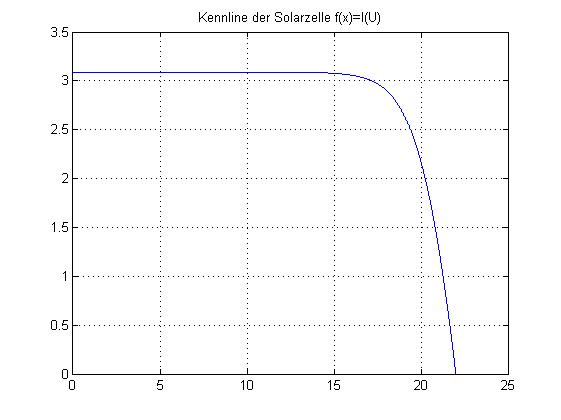
\includegraphics[width=0.9\textwidth]{Kennlinie.jpg}
	\caption{Die Kennlinie, welche mittels der Formeln ermittelt wurde.}
	\label{fig:Kennlinie}
\end{figure}
\begin{figure}
	\centering
		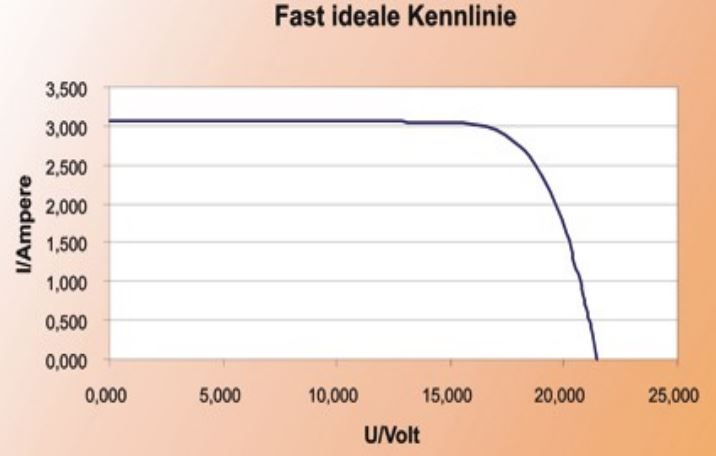
\includegraphics[width=0.60\textwidth]{Kennlinie_Lastenheft.jpg}
	\caption{Die Kennlinie, welche mittels der Formeln ermittelt wurde.}
	\label{fig:Kennlinie_Lastenheft}
\end{figure}

\subsubsection{Anpassung der Kennlinie bei verschiedenen Bestrahlungsstärken}
Gemäss dem Lastenheft soll es ausserdem möglich sein, die Bestrahlungsstärke in einem Wertebereich von 20\% bis 100\% einstellen zu können. Bei Abnahme der Bestrahlung verschiebt sich die Kennlinie nach unten, sodass der Stromwert folgendermassen angepasst werden muss:
\begin{equation}
	I_{neu}=I+\frac{100-\left[\text{Bestrahlungsstärke in Prozent}\right]}{100}\cdot I_{SC}
\label{eq:kennlinie_prozent}
\end{equation}
Beispielhaft wurden mittels Matlab zwei zusätzliche Kennlinien für 60\% und 20\% dargestellt, zu sehen in Abbildung \ref{fig:Kennlinie_Auslastung}. Die beiden Kennlinien bei verringerter Bestrahlungsstärke verhalten sich bei $I_{neu}>I_{SC}$ unerwünscht, im Programm selbst wird dies jedoch mittels einer if-Prüfung verhindert.
\begin{figure}
	\centering
		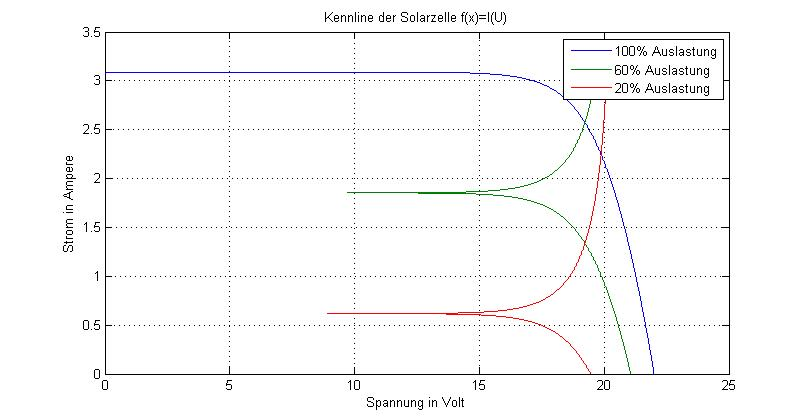
\includegraphics[width=0.9\textwidth]{Kennlinie_Auslastung.jpg}
	\caption{Verhalten der Kennlinie bei verschiedenen Bestrahlungsstärken.}
	\label{fig:Kennlinie_Auslastung}
\end{figure}
